
%(BEGIN_QUESTION)
% Copyright 2014, Tony R. Kuphaldt, released under the Creative Commons Attribution License (v 1.0)
% This means you may do almost anything with this work of mine, so long as you give me proper credit

Anta at du må måle spenningsutgangen fra en kombinasjons-pH-elektrode i en væske, men bare har standard DMM-er. Du vet at ``null-balance''/``potensiometrisk'' metode kan brukes selv med lavimpedante målere. Skisser en null-balance krets koblet til pH-proben. Du kan legge til passive komponenter ved behov:

$$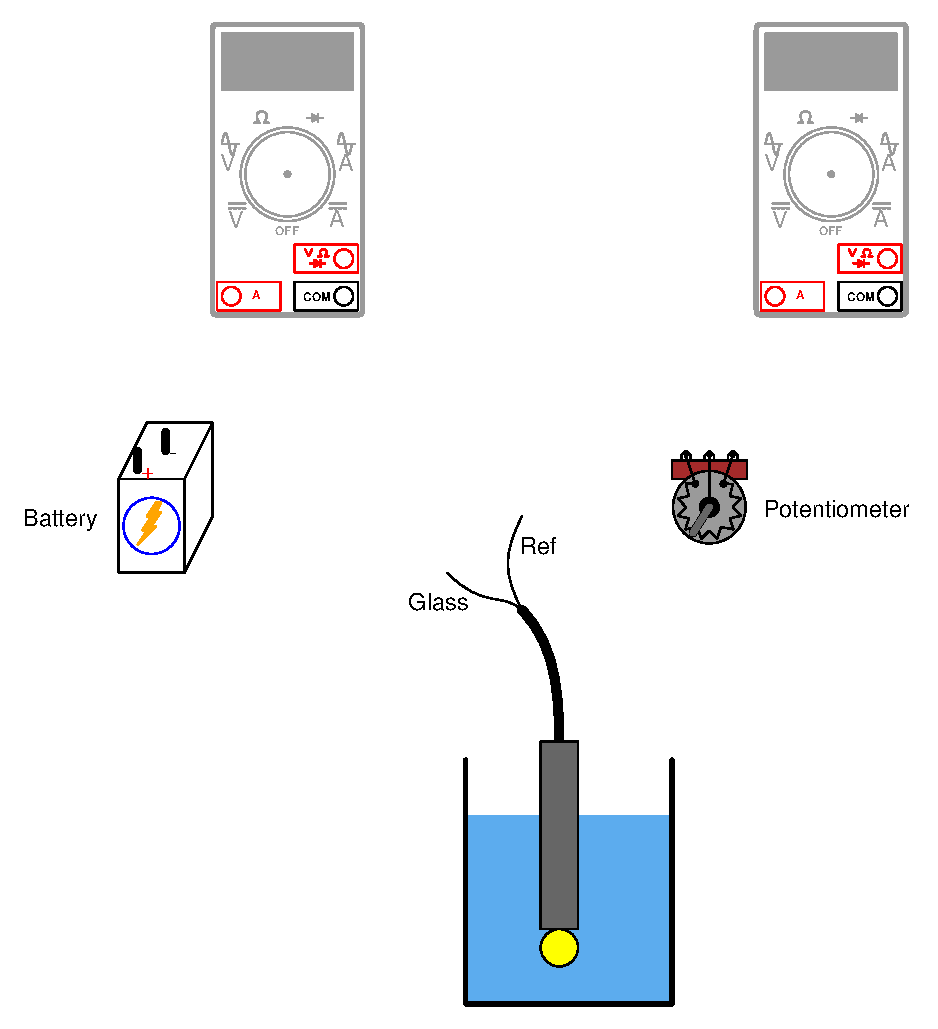
\includegraphics[width=15.5cm]{i00965x01.eps}$$

Forklar også hvorfor null-balance virker for pH-probe, mens en direktekoblet DMM gir feil måling.

\underbar{file i00965}
%(END_QUESTION)





%(BEGIN_ANSWER)

5 poeng for riktig skisse, 5 poeng for forklaring:

\vskip 10pt

Flere løsninger er mulige, men voltmeter må ligge parallelt med justerbar DC-spenning, og ammeter i serie med pH-proben for å indikere null strøm.
 
$$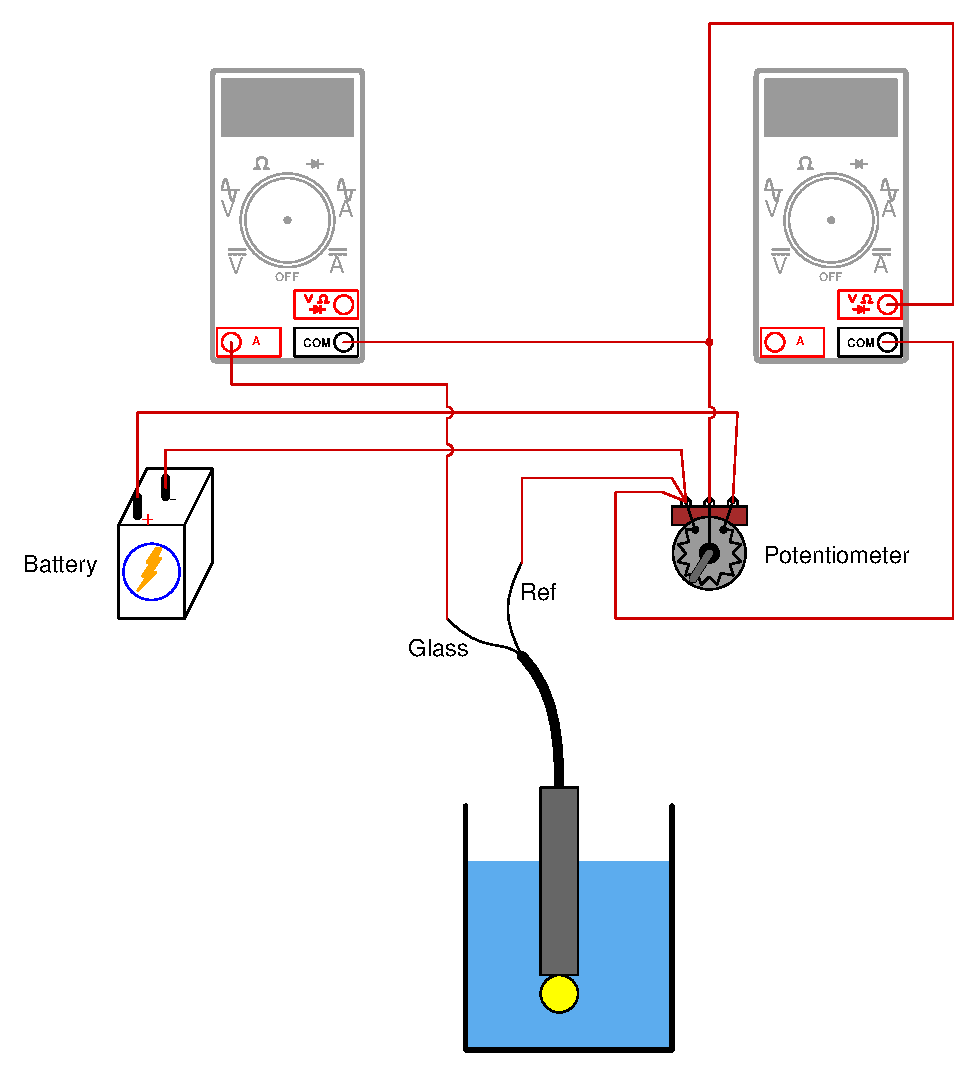
\includegraphics[width=15.5cm]{i00965x02.eps}$$

\vskip 10pt

Null-balance sikrer at ingen strøm trekkes fra spenningskilden under test (pH-proben). Uten strømtrekk blir kildeimpedansen irrelevant. Direktekoblet DMM belaster høyimpedant kilde og gir for lav avlesning.

%(END_ANSWER)





%(BEGIN_NOTES)

{\bf Denne oppgaven er ment kun for eksamen, ikke for arbeidsark!}.

%(END_NOTES)

